\documentclass[twoside]{book}

% Packages required by doxygen
\usepackage{calc}
\usepackage{doxygen}
\usepackage{graphicx}
\usepackage[utf8]{inputenc}
\usepackage{makeidx}
\usepackage{multicol}
\usepackage{multirow}
\usepackage{fixltx2e}
\PassOptionsToPackage{warn}{textcomp}
\usepackage{textcomp}
\usepackage[nointegrals]{wasysym}
\usepackage[table]{xcolor}

% Font selection
\usepackage[T1]{fontenc}
\usepackage{mathptmx}
\usepackage[scaled=.90]{helvet}
\usepackage{courier}
\usepackage{amssymb}
\usepackage{sectsty}
\renewcommand{\familydefault}{\sfdefault}
\allsectionsfont{%
  \fontseries{bc}\selectfont%
  \color{darkgray}%
}
\renewcommand{\DoxyLabelFont}{%
  \fontseries{bc}\selectfont%
  \color{darkgray}%
}
\newcommand{\+}{\discretionary{\mbox{\scriptsize$\hookleftarrow$}}{}{}}

% Page & text layout
\usepackage{geometry}
\geometry{%
  a4paper,%
  top=2.5cm,%
  bottom=2.5cm,%
  left=2.5cm,%
  right=2.5cm%
}
\tolerance=750
\hfuzz=15pt
\hbadness=750
\setlength{\emergencystretch}{15pt}
\setlength{\parindent}{0cm}
\setlength{\parskip}{0.2cm}
\makeatletter
\renewcommand{\paragraph}{%
  \@startsection{paragraph}{4}{0ex}{-1.0ex}{1.0ex}{%
    \normalfont\normalsize\bfseries\SS@parafont%
  }%
}
\renewcommand{\subparagraph}{%
  \@startsection{subparagraph}{5}{0ex}{-1.0ex}{1.0ex}{%
    \normalfont\normalsize\bfseries\SS@subparafont%
  }%
}
\makeatother

% Headers & footers
\usepackage{fancyhdr}
\pagestyle{fancyplain}
\fancyhead[LE]{\fancyplain{}{\bfseries\thepage}}
\fancyhead[CE]{\fancyplain{}{}}
\fancyhead[RE]{\fancyplain{}{\bfseries\leftmark}}
\fancyhead[LO]{\fancyplain{}{\bfseries\rightmark}}
\fancyhead[CO]{\fancyplain{}{}}
\fancyhead[RO]{\fancyplain{}{\bfseries\thepage}}
\fancyfoot[LE]{\fancyplain{}{}}
\fancyfoot[CE]{\fancyplain{}{}}
\fancyfoot[RE]{\fancyplain{}{\bfseries\scriptsize Generated on Sun Jul 20 2014 21\+:12\+:04 for Hesed by Doxygen }}
\fancyfoot[LO]{\fancyplain{}{\bfseries\scriptsize Generated on Sun Jul 20 2014 21\+:12\+:04 for Hesed by Doxygen }}
\fancyfoot[CO]{\fancyplain{}{}}
\fancyfoot[RO]{\fancyplain{}{}}
\renewcommand{\footrulewidth}{0.4pt}
\renewcommand{\chaptermark}[1]{%
  \markboth{#1}{}%
}
\renewcommand{\sectionmark}[1]{%
  \markright{\thesection\ #1}%
}

% Indices & bibliography
\usepackage{natbib}
\usepackage[titles]{tocloft}
\setcounter{tocdepth}{3}
\setcounter{secnumdepth}{5}
\makeindex

% Hyperlinks (required, but should be loaded last)
\usepackage{ifpdf}
\ifpdf
  \usepackage[pdftex,pagebackref=true]{hyperref}
\else
  \usepackage[ps2pdf,pagebackref=true]{hyperref}
\fi
\hypersetup{%
  colorlinks=true,%
  linkcolor=blue,%
  citecolor=blue,%
  unicode%
}

% Custom commands
\newcommand{\clearemptydoublepage}{%
  \newpage{\pagestyle{empty}\cleardoublepage}%
}


%===== C O N T E N T S =====

\begin{document}

% Titlepage & ToC
\hypersetup{pageanchor=false,
             bookmarks=true,
             bookmarksnumbered=true,
             pdfencoding=unicode
            }
\pagenumbering{roman}
\begin{titlepage}
\vspace*{7cm}
\begin{center}%
{\Large Hesed \\[1ex]\large version 0.\+1 }\\
\vspace*{1cm}
{\large Generated by Doxygen 1.8.7}\\
\vspace*{0.5cm}
{\small Sun Jul 20 2014 21:12:04}\\
\end{center}
\end{titlepage}
\clearemptydoublepage
\tableofcontents
\clearemptydoublepage
\pagenumbering{arabic}
\hypersetup{pageanchor=true}

%--- Begin generated contents ---
\chapter{Namespace Index}
\input{namespaces}
\chapter{Hierarchical Index}
\section{Class Hierarchy}
This inheritance list is sorted roughly, but not completely, alphabetically\+:\begin{DoxyCompactList}
\item \contentsline{section}{Person\+:\+:info}{\pageref{struct_person_1_1info}}{}
\item \contentsline{section}{Person}{\pageref{class_person}}{}
\item Q\+Main\+Window\begin{DoxyCompactList}
\item \contentsline{section}{Main\+Window}{\pageref{class_main_window}}{}
\end{DoxyCompactList}
\end{DoxyCompactList}

\chapter{Class Index}
\section{Class List}
Here are the classes, structs, unions and interfaces with brief descriptions\+:\begin{DoxyCompactList}
\item\contentsline{section}{\hyperlink{class_main_window}{Main\+Window} }{\pageref{class_main_window}}{}
\item\contentsline{section}{\hyperlink{class_person}{Person} }{\pageref{class_person}}{}
\end{DoxyCompactList}

\chapter{File Index}
\section{File List}
Here is a list of all files with brief descriptions\+:\begin{DoxyCompactList}
\item\contentsline{section}{\hyperlink{dialog_8cpp}{dialog.\+cpp} }{\pageref{dialog_8cpp}}{}
\item\contentsline{section}{\hyperlink{dialog_8h}{dialog.\+h} }{\pageref{dialog_8h}}{}
\item\contentsline{section}{\hyperlink{info_8h}{info.\+h} }{\pageref{info_8h}}{}
\item\contentsline{section}{\hyperlink{main_8cpp}{main.\+cpp} }{\pageref{main_8cpp}}{}
\item\contentsline{section}{\hyperlink{mainwindow_8cpp}{mainwindow.\+cpp} }{\pageref{mainwindow_8cpp}}{}
\item\contentsline{section}{\hyperlink{mainwindow_8h}{mainwindow.\+h} }{\pageref{mainwindow_8h}}{}
\item\contentsline{section}{\hyperlink{person_8cpp}{person.\+cpp} }{\pageref{person_8cpp}}{}
\item\contentsline{section}{\hyperlink{person_8h}{person.\+h} }{\pageref{person_8h}}{}
\end{DoxyCompactList}

\chapter{Namespace Documentation}
\hypertarget{namespace_ui}{\section{Ui Namespace Reference}
\label{namespace_ui}\index{Ui@{Ui}}
}

\chapter{Class Documentation}
\hypertarget{struct_person_1_1info}{\section{Person\+:\+:info Struct Reference}
\label{struct_person_1_1info}\index{Person\+::info@{Person\+::info}}
}


Struct to store basic people information.  


\subsection*{Public Attributes}
\begin{DoxyCompactItemize}
\item 
Q\+String \hyperlink{struct_person_1_1info_a81051c5b2abdf064395938f2f47017b8}{name}
\begin{DoxyCompactList}\small\item\em Name. \end{DoxyCompactList}\item 
Q\+String \hyperlink{struct_person_1_1info_a5dffef4c24ab24eaa62a3428e04b4239}{surname}
\begin{DoxyCompactList}\small\item\em Surname. \end{DoxyCompactList}\item 
Q\+String \hyperlink{struct_person_1_1info_ab91922388b5ba74969a7d8f7a4fad95b}{N\+I\+F}
\begin{DoxyCompactList}\small\item\em Personal N\+I\+F (Número de Identificación Fiscal) \end{DoxyCompactList}\item 
Q\+String \hyperlink{struct_person_1_1info_a3ee6bcba23c2257f4571084e7a734e6d}{c\+N\+I\+F}
\begin{DoxyCompactList}\small\item\em Couple N\+I\+F (Número de Identificación Fiscal) \end{DoxyCompactList}\item 
Q\+String \hyperlink{struct_person_1_1info_a350817c964e878c2c59019eb51e9f608}{adress}
\begin{DoxyCompactList}\small\item\em Personal home adress. \end{DoxyCompactList}\item 
Q\+String \hyperlink{struct_person_1_1info_a07a8d88e73398595a0e0282eaffe9fef}{phone}
\begin{DoxyCompactList}\small\item\em Personal phone. \end{DoxyCompactList}\item 
Q\+Date \hyperlink{struct_person_1_1info_a803a2ee586aaa2503e10447b1435e916}{birth\+Date}
\begin{DoxyCompactList}\small\item\em Date of birth. \end{DoxyCompactList}\item 
Q\+Date \hyperlink{struct_person_1_1info_a835c907e641433331e06c62bcde9dfe9}{begin\+Help}
\begin{DoxyCompactList}\small\item\em First day recieved help. \end{DoxyCompactList}\item 
Q\+Date \hyperlink{struct_person_1_1info_acc738154c5e01adc22c880fc49d6e09c}{end\+Help}
\begin{DoxyCompactList}\small\item\em Finishing help date. \end{DoxyCompactList}\item 
int \hyperlink{struct_person_1_1info_a6fd0e334bf6cc9baf667ef94806ed993}{number\+Help}
\begin{DoxyCompactList}\small\item\em Number of times that somebody has been helped. \end{DoxyCompactList}\item 
int \hyperlink{struct_person_1_1info_afc121f83e810c2c0318e115f4ba6d730}{fam\+Members}
\begin{DoxyCompactList}\small\item\em Amount of members in the home family. \end{DoxyCompactList}\item 
unsigned int \hyperlink{struct_person_1_1info_a535ca27747d371eb58005194190f6bd6}{I\+D}
\begin{DoxyCompactList}\small\item\em Identification number for internal use. \end{DoxyCompactList}\end{DoxyCompactItemize}


\subsection{Detailed Description}
Struct to store basic people information. 

Stored info is\+: 
\begin{DoxyItemize}
\item Name 
\item Surname 
\item N\+I\+F 
\item Birth Date 
\item Couple N\+I\+F 
\item Adress 
\item Phone number 
\item Start help date 
\item End help date 
\item Times helped 
\item Identification Number 
\item Family members 
\end{DoxyItemize}

Definition at line 36 of file person.\+h.



\subsection{Member Data Documentation}
\hypertarget{struct_person_1_1info_a81051c5b2abdf064395938f2f47017b8}{\index{Person\+::info@{Person\+::info}!name@{name}}
\index{name@{name}!Person\+::info@{Person\+::info}}
\subsubsection[{name}]{\setlength{\rightskip}{0pt plus 5cm}Person\+::info\+::name}}\label{struct_person_1_1info_a81051c5b2abdf064395938f2f47017b8}


Name. 



Definition at line 51 of file person.\+h.

\hypertarget{struct_person_1_1info_a5dffef4c24ab24eaa62a3428e04b4239}{\index{Person\+::info@{Person\+::info}!surname@{surname}}
\index{surname@{surname}!Person\+::info@{Person\+::info}}
\subsubsection[{surname}]{\setlength{\rightskip}{0pt plus 5cm}Person\+::info\+::surname}}\label{struct_person_1_1info_a5dffef4c24ab24eaa62a3428e04b4239}


Surname. 



Definition at line 51 of file person.\+h.

\hypertarget{struct_person_1_1info_ab91922388b5ba74969a7d8f7a4fad95b}{\index{Person\+::info@{Person\+::info}!N\+I\+F@{N\+I\+F}}
\index{N\+I\+F@{N\+I\+F}!Person\+::info@{Person\+::info}}
\subsubsection[{N\+I\+F}]{\setlength{\rightskip}{0pt plus 5cm}Person\+::info\+::\+N\+I\+F}}\label{struct_person_1_1info_ab91922388b5ba74969a7d8f7a4fad95b}


Personal N\+I\+F (Número de Identificación Fiscal) 



Definition at line 51 of file person.\+h.

\hypertarget{struct_person_1_1info_a3ee6bcba23c2257f4571084e7a734e6d}{\index{Person\+::info@{Person\+::info}!c\+N\+I\+F@{c\+N\+I\+F}}
\index{c\+N\+I\+F@{c\+N\+I\+F}!Person\+::info@{Person\+::info}}
\subsubsection[{c\+N\+I\+F}]{\setlength{\rightskip}{0pt plus 5cm}Person\+::info\+::c\+N\+I\+F}}\label{struct_person_1_1info_a3ee6bcba23c2257f4571084e7a734e6d}


Couple N\+I\+F (Número de Identificación Fiscal) 



Definition at line 51 of file person.\+h.

\hypertarget{struct_person_1_1info_a350817c964e878c2c59019eb51e9f608}{\index{Person\+::info@{Person\+::info}!adress@{adress}}
\index{adress@{adress}!Person\+::info@{Person\+::info}}
\subsubsection[{adress}]{\setlength{\rightskip}{0pt plus 5cm}Person\+::info\+::adress}}\label{struct_person_1_1info_a350817c964e878c2c59019eb51e9f608}


Personal home adress. 



Definition at line 51 of file person.\+h.

\hypertarget{struct_person_1_1info_a07a8d88e73398595a0e0282eaffe9fef}{\index{Person\+::info@{Person\+::info}!phone@{phone}}
\index{phone@{phone}!Person\+::info@{Person\+::info}}
\subsubsection[{phone}]{\setlength{\rightskip}{0pt plus 5cm}Person\+::info\+::phone}}\label{struct_person_1_1info_a07a8d88e73398595a0e0282eaffe9fef}


Personal phone. 



Definition at line 51 of file person.\+h.

\hypertarget{struct_person_1_1info_a803a2ee586aaa2503e10447b1435e916}{\index{Person\+::info@{Person\+::info}!birth\+Date@{birth\+Date}}
\index{birth\+Date@{birth\+Date}!Person\+::info@{Person\+::info}}
\subsubsection[{birth\+Date}]{\setlength{\rightskip}{0pt plus 5cm}Person\+::info\+::birth\+Date}}\label{struct_person_1_1info_a803a2ee586aaa2503e10447b1435e916}


Date of birth. 



Definition at line 60 of file person.\+h.

\hypertarget{struct_person_1_1info_a835c907e641433331e06c62bcde9dfe9}{\index{Person\+::info@{Person\+::info}!begin\+Help@{begin\+Help}}
\index{begin\+Help@{begin\+Help}!Person\+::info@{Person\+::info}}
\subsubsection[{begin\+Help}]{\setlength{\rightskip}{0pt plus 5cm}Person\+::info\+::begin\+Help}}\label{struct_person_1_1info_a835c907e641433331e06c62bcde9dfe9}


First day recieved help. 



Definition at line 60 of file person.\+h.

\hypertarget{struct_person_1_1info_acc738154c5e01adc22c880fc49d6e09c}{\index{Person\+::info@{Person\+::info}!end\+Help@{end\+Help}}
\index{end\+Help@{end\+Help}!Person\+::info@{Person\+::info}}
\subsubsection[{end\+Help}]{\setlength{\rightskip}{0pt plus 5cm}Person\+::info\+::end\+Help}}\label{struct_person_1_1info_acc738154c5e01adc22c880fc49d6e09c}


Finishing help date. 



Definition at line 60 of file person.\+h.

\hypertarget{struct_person_1_1info_a6fd0e334bf6cc9baf667ef94806ed993}{\index{Person\+::info@{Person\+::info}!number\+Help@{number\+Help}}
\index{number\+Help@{number\+Help}!Person\+::info@{Person\+::info}}
\subsubsection[{number\+Help}]{\setlength{\rightskip}{0pt plus 5cm}Person\+::info\+::number\+Help}}\label{struct_person_1_1info_a6fd0e334bf6cc9baf667ef94806ed993}


Number of times that somebody has been helped. 



Definition at line 67 of file person.\+h.

\hypertarget{struct_person_1_1info_afc121f83e810c2c0318e115f4ba6d730}{\index{Person\+::info@{Person\+::info}!fam\+Members@{fam\+Members}}
\index{fam\+Members@{fam\+Members}!Person\+::info@{Person\+::info}}
\subsubsection[{fam\+Members}]{\setlength{\rightskip}{0pt plus 5cm}Person\+::info\+::fam\+Members}}\label{struct_person_1_1info_afc121f83e810c2c0318e115f4ba6d730}


Amount of members in the home family. 



Definition at line 67 of file person.\+h.

\hypertarget{struct_person_1_1info_a535ca27747d371eb58005194190f6bd6}{\index{Person\+::info@{Person\+::info}!I\+D@{I\+D}}
\index{I\+D@{I\+D}!Person\+::info@{Person\+::info}}
\subsubsection[{I\+D}]{\setlength{\rightskip}{0pt plus 5cm}Person\+::info\+::\+I\+D}}\label{struct_person_1_1info_a535ca27747d371eb58005194190f6bd6}


Identification number for internal use. 



Definition at line 72 of file person.\+h.



The documentation for this struct was generated from the following file\+:\begin{DoxyCompactItemize}
\item 
\hyperlink{person_8h}{person.\+h}\end{DoxyCompactItemize}

\hypertarget{class_main_window}{\section{Main\+Window Class Reference}
\label{class_main_window}\index{Main\+Window@{Main\+Window}}
}


Class to show basic information to user.  


\subsection*{Public Member Functions}
\begin{DoxyCompactItemize}
\item 
\hyperlink{class_main_window_a8b244be8b7b7db1b08de2a2acb9409db}{Main\+Window} (Q\+Widget $\ast$parent=0)
\begin{DoxyCompactList}\small\item\em Default constructor. \end{DoxyCompactList}\item 
\hyperlink{class_main_window_ae98d00a93bc118200eeef9f9bba1dba7}{$\sim$\+Main\+Window} ()
\item 
void \hyperlink{class_main_window_a6906cd747941813c6da899b18d881473}{load\+Data} ()
\begin{DoxyCompactList}\small\item\em Function that loads data when exists de {\itshape Data} folder. \end{DoxyCompactList}\item 
void \hyperlink{class_main_window_a44d044deed1ddca8952f59554705e28d}{add\+Path} (const Q\+Dir \&\hyperlink{class_main_window_a1dc35bda22acc11636be809539ab73d9}{data})
\begin{DoxyCompactList}\small\item\em Function to add the {\itshape Data} folder path. \end{DoxyCompactList}\end{DoxyCompactItemize}
\subsection*{Private Slots}
\begin{DoxyCompactItemize}
\item 
void \hyperlink{class_main_window_a308a629f351133027a3602d27099cb7c}{on\+\_\+action\+Inserir\+\_\+triggered} ()
\item 
void \hyperlink{class_main_window_a0ab4c2fb4c79e29566e20a0ee60edf77}{end\+Inserir} ()
\end{DoxyCompactItemize}
\subsection*{Private Attributes}
\begin{DoxyCompactItemize}
\item 
Q\+Dir \hyperlink{class_main_window_a1dc35bda22acc11636be809539ab73d9}{data}
\item 
Ui\+::\+Main\+Window $\ast$ \hyperlink{class_main_window_a35466a70ed47252a0191168126a352a5}{ui}
\item 
\hyperlink{class_person}{Person} \hyperlink{class_main_window_a2d1f101eed410e692b5db9b7226174bf}{info}
\item 
\hyperlink{class_ins_dialog}{Ins\+Dialog} $\ast$ \hyperlink{class_main_window_ad84bd8f23d732609dc5a01cbe3ae21de}{inf}
\end{DoxyCompactItemize}


\subsection{Detailed Description}
Class to show basic information to user. 

Definition at line 17 of file mainwindow.\+h.



\subsection{Constructor \& Destructor Documentation}
\hypertarget{class_main_window_a8b244be8b7b7db1b08de2a2acb9409db}{\index{Main\+Window@{Main\+Window}!Main\+Window@{Main\+Window}}
\index{Main\+Window@{Main\+Window}!Main\+Window@{Main\+Window}}
\subsubsection[{Main\+Window}]{\setlength{\rightskip}{0pt plus 5cm}Main\+Window\+::\+Main\+Window (
\begin{DoxyParamCaption}
\item[{Q\+Widget $\ast$}]{parent = {\ttfamily 0}}
\end{DoxyParamCaption}
)\hspace{0.3cm}{\ttfamily [explicit]}}}\label{class_main_window_a8b244be8b7b7db1b08de2a2acb9409db}


Default constructor. 


\begin{DoxyParams}{Parameters}
{\em parent} & Default parameter \\
\hline
\end{DoxyParams}


Definition at line 9 of file mainwindow.\+cpp.


\begin{DoxyCode}
9                                      :QMainWindow(parent),
10     \hyperlink{class_main_window_a35466a70ed47252a0191168126a352a5}{ui}(\textcolor{keyword}{new} Ui::MainWindow)
11 \{
12     \hyperlink{class_main_window_a35466a70ed47252a0191168126a352a5}{ui}->setupUi(\textcolor{keyword}{this});
13 \}
\end{DoxyCode}
\hypertarget{class_main_window_ae98d00a93bc118200eeef9f9bba1dba7}{\index{Main\+Window@{Main\+Window}!````~Main\+Window@{$\sim$\+Main\+Window}}
\index{````~Main\+Window@{$\sim$\+Main\+Window}!Main\+Window@{Main\+Window}}
\subsubsection[{$\sim$\+Main\+Window}]{\setlength{\rightskip}{0pt plus 5cm}Main\+Window\+::$\sim$\+Main\+Window (
\begin{DoxyParamCaption}
{}
\end{DoxyParamCaption}
)}}\label{class_main_window_ae98d00a93bc118200eeef9f9bba1dba7}


Definition at line 15 of file mainwindow.\+cpp.


\begin{DoxyCode}
16 \{
17     \textcolor{keyword}{delete} \hyperlink{class_main_window_a35466a70ed47252a0191168126a352a5}{ui};
18 \}
\end{DoxyCode}


\subsection{Member Function Documentation}
\hypertarget{class_main_window_a6906cd747941813c6da899b18d881473}{\index{Main\+Window@{Main\+Window}!load\+Data@{load\+Data}}
\index{load\+Data@{load\+Data}!Main\+Window@{Main\+Window}}
\subsubsection[{load\+Data}]{\setlength{\rightskip}{0pt plus 5cm}void Main\+Window\+::load\+Data (
\begin{DoxyParamCaption}
{}
\end{DoxyParamCaption}
)}}\label{class_main_window_a6906cd747941813c6da899b18d881473}


Function that loads data when exists de {\itshape Data} folder. 



Definition at line 24 of file mainwindow.\+cpp.


\begin{DoxyCode}
25 \{
26     \hyperlink{class_main_window_a2d1f101eed410e692b5db9b7226174bf}{info}.\hyperlink{class_person_a98c73f33a51b80cc9296a949f2fc5cf3}{read}(\hyperlink{class_main_window_a1dc35bda22acc11636be809539ab73d9}{data});
27     \hyperlink{class_main_window_a2d1f101eed410e692b5db9b7226174bf}{info}.\hyperlink{class_person_a100215914f651662a6207722ef28769e}{addTable}(\hyperlink{class_main_window_a35466a70ed47252a0191168126a352a5}{ui}->tableView);
28     \hyperlink{class_main_window_a2d1f101eed410e692b5db9b7226174bf}{info}.\hyperlink{class_person_a2f1231629a6e7e8c83ada57628e80a89}{show}();
29 \}
\end{DoxyCode}
\hypertarget{class_main_window_a44d044deed1ddca8952f59554705e28d}{\index{Main\+Window@{Main\+Window}!add\+Path@{add\+Path}}
\index{add\+Path@{add\+Path}!Main\+Window@{Main\+Window}}
\subsubsection[{add\+Path}]{\setlength{\rightskip}{0pt plus 5cm}void Main\+Window\+::add\+Path (
\begin{DoxyParamCaption}
\item[{const Q\+Dir \&}]{data}
\end{DoxyParamCaption}
)}}\label{class_main_window_a44d044deed1ddca8952f59554705e28d}


Function to add the {\itshape Data} folder path. 


\begin{DoxyParams}{Parameters}
{\em data} & Contains de P\+A\+T\+H to de {\itshape Data} folder. \\
\hline
\end{DoxyParams}


Definition at line 31 of file mainwindow.\+cpp.


\begin{DoxyCode}
32 \{
33     this->\hyperlink{class_main_window_a1dc35bda22acc11636be809539ab73d9}{data} = \hyperlink{class_main_window_a1dc35bda22acc11636be809539ab73d9}{data};
34 \}
\end{DoxyCode}
\hypertarget{class_main_window_a308a629f351133027a3602d27099cb7c}{\index{Main\+Window@{Main\+Window}!on\+\_\+action\+Inserir\+\_\+triggered@{on\+\_\+action\+Inserir\+\_\+triggered}}
\index{on\+\_\+action\+Inserir\+\_\+triggered@{on\+\_\+action\+Inserir\+\_\+triggered}!Main\+Window@{Main\+Window}}
\subsubsection[{on\+\_\+action\+Inserir\+\_\+triggered}]{\setlength{\rightskip}{0pt plus 5cm}void Main\+Window\+::on\+\_\+action\+Inserir\+\_\+triggered (
\begin{DoxyParamCaption}
{}
\end{DoxyParamCaption}
)\hspace{0.3cm}{\ttfamily [private]}, {\ttfamily [slot]}}}\label{class_main_window_a308a629f351133027a3602d27099cb7c}


Definition at line 36 of file mainwindow.\+cpp.


\begin{DoxyCode}
37 \{
38     \hyperlink{class_main_window_ad84bd8f23d732609dc5a01cbe3ae21de}{inf} = \textcolor{keyword}{new} \hyperlink{class_ins_dialog}{InsDialog};
39     \hyperlink{class_main_window_ad84bd8f23d732609dc5a01cbe3ae21de}{inf}->setWindowTitle(\textcolor{stringliteral}{"Associació Hesed - Inserir"});
40     \hyperlink{class_main_window_ad84bd8f23d732609dc5a01cbe3ae21de}{inf}->open();
41     connect(\hyperlink{class_main_window_ad84bd8f23d732609dc5a01cbe3ae21de}{inf}, SIGNAL(accepted()), \textcolor{keyword}{this}, SLOT(\hyperlink{class_main_window_a0ab4c2fb4c79e29566e20a0ee60edf77}{endInserir}()));
42     connect(\hyperlink{class_main_window_ad84bd8f23d732609dc5a01cbe3ae21de}{inf}, SIGNAL(rejected()), \textcolor{keyword}{this}, SLOT(\hyperlink{class_main_window_a0ab4c2fb4c79e29566e20a0ee60edf77}{endInserir}()));
43     
44 \}
\end{DoxyCode}
\hypertarget{class_main_window_a0ab4c2fb4c79e29566e20a0ee60edf77}{\index{Main\+Window@{Main\+Window}!end\+Inserir@{end\+Inserir}}
\index{end\+Inserir@{end\+Inserir}!Main\+Window@{Main\+Window}}
\subsubsection[{end\+Inserir}]{\setlength{\rightskip}{0pt plus 5cm}void Main\+Window\+::end\+Inserir (
\begin{DoxyParamCaption}
{}
\end{DoxyParamCaption}
)\hspace{0.3cm}{\ttfamily [private]}, {\ttfamily [slot]}}}\label{class_main_window_a0ab4c2fb4c79e29566e20a0ee60edf77}


Definition at line 46 of file mainwindow.\+cpp.


\begin{DoxyCode}
47 \{
48     \textcolor{keywordflow}{if} (\hyperlink{class_main_window_ad84bd8f23d732609dc5a01cbe3ae21de}{inf}->result()) \{
49         qDebug() << \textcolor{stringliteral}{"Acceptat"};
50     \}
51     \textcolor{keywordflow}{else} qDebug() << \textcolor{stringliteral}{"No acceptat"};
52     \textcolor{keyword}{delete} \hyperlink{class_main_window_ad84bd8f23d732609dc5a01cbe3ae21de}{inf};    
53 \}
\end{DoxyCode}


\subsection{Member Data Documentation}
\hypertarget{class_main_window_a1dc35bda22acc11636be809539ab73d9}{\index{Main\+Window@{Main\+Window}!data@{data}}
\index{data@{data}!Main\+Window@{Main\+Window}}
\subsubsection[{data}]{\setlength{\rightskip}{0pt plus 5cm}Q\+Dir Main\+Window\+::data\hspace{0.3cm}{\ttfamily [private]}}}\label{class_main_window_a1dc35bda22acc11636be809539ab73d9}


Definition at line 55 of file mainwindow.\+h.

\hypertarget{class_main_window_a35466a70ed47252a0191168126a352a5}{\index{Main\+Window@{Main\+Window}!ui@{ui}}
\index{ui@{ui}!Main\+Window@{Main\+Window}}
\subsubsection[{ui}]{\setlength{\rightskip}{0pt plus 5cm}Ui\+::\+Main\+Window$\ast$ Main\+Window\+::ui\hspace{0.3cm}{\ttfamily [private]}}}\label{class_main_window_a35466a70ed47252a0191168126a352a5}


Definition at line 56 of file mainwindow.\+h.

\hypertarget{class_main_window_a2d1f101eed410e692b5db9b7226174bf}{\index{Main\+Window@{Main\+Window}!info@{info}}
\index{info@{info}!Main\+Window@{Main\+Window}}
\subsubsection[{info}]{\setlength{\rightskip}{0pt plus 5cm}{\bf Person} Main\+Window\+::info\hspace{0.3cm}{\ttfamily [private]}}}\label{class_main_window_a2d1f101eed410e692b5db9b7226174bf}


Definition at line 57 of file mainwindow.\+h.

\hypertarget{class_main_window_ad84bd8f23d732609dc5a01cbe3ae21de}{\index{Main\+Window@{Main\+Window}!inf@{inf}}
\index{inf@{inf}!Main\+Window@{Main\+Window}}
\subsubsection[{inf}]{\setlength{\rightskip}{0pt plus 5cm}{\bf Ins\+Dialog}$\ast$ Main\+Window\+::inf\hspace{0.3cm}{\ttfamily [private]}}}\label{class_main_window_ad84bd8f23d732609dc5a01cbe3ae21de}


Definition at line 58 of file mainwindow.\+h.



The documentation for this class was generated from the following files\+:\begin{DoxyCompactItemize}
\item 
\hyperlink{mainwindow_8h}{mainwindow.\+h}\item 
\hyperlink{mainwindow_8cpp}{mainwindow.\+cpp}\end{DoxyCompactItemize}

\hypertarget{class_person}{\section{Person Class Reference}
\label{class_person}\index{Person@{Person}}
}


The \hyperlink{class_person}{Person} Class contains all people basic data.  


\subsection*{Classes}
\begin{DoxyCompactItemize}
\item 
struct \hyperlink{struct_person_1_1comp}{comp}
\begin{DoxyCompactList}\small\item\em The comp struct is used to sort the info. \end{DoxyCompactList}\end{DoxyCompactItemize}
\subsection*{Public Member Functions}
\begin{DoxyCompactItemize}
\item 
\hyperlink{class_person_a0397c6f89fafc12e738923f612bc41a3}{Person} ()
\begin{DoxyCompactList}\small\item\em Default constructor. \end{DoxyCompactList}\item 
\hyperlink{class_person_a847845e2e214a89e790c584678f1ea97}{Person} (const \hyperlink{class_person}{Person} \&p)
\begin{DoxyCompactList}\small\item\em Copy constructor. \end{DoxyCompactList}\item 
void \hyperlink{class_person_a98c73f33a51b80cc9296a949f2fc5cf3}{read} (Q\+Dir data)
\begin{DoxyCompactList}\small\item\em Function to read all stored data. \end{DoxyCompactList}\item 
void \hyperlink{class_person_aa667ce32c0552e818ac6df14c9a5f50d}{write} (Q\+Dir data)
\begin{DoxyCompactList}\small\item\em Function to store all data to a file. \end{DoxyCompactList}\item 
void \hyperlink{class_person_a602ce88a8ef959c3f4044d9dc00dd2cf}{sort} (int type)
\begin{DoxyCompactList}\small\item\em Function to sort the data with the specified metod. \end{DoxyCompactList}\item 
void \hyperlink{class_person_a100215914f651662a6207722ef28769e}{add\+Table} (Q\+Table\+View $\ast$t)
\begin{DoxyCompactList}\small\item\em Adds the pointer to a Q\+Table\+View. \end{DoxyCompactList}\item 
void \hyperlink{class_person_a1f2447001ce07f9d5d6b1a7a5da29198}{add\+Info} ()
\item 
void \hyperlink{class_person_a2f1231629a6e7e8c83ada57628e80a89}{show} ()
\begin{DoxyCompactList}\small\item\em Function to show all stored data. \end{DoxyCompactList}\end{DoxyCompactItemize}
\subsection*{Private Attributes}
\begin{DoxyCompactItemize}
\item 
list$<$ \hyperlink{structinfo}{info} $>$ \hyperlink{class_person_a23d6ff8cb8e45c9e3502baffa6a0468a}{all}
\begin{DoxyCompactList}\small\item\em List to store all data. \end{DoxyCompactList}\item 
unsigned int \hyperlink{class_person_a816ee6194426eb703b61ae267e8e8ee6}{max\+I\+D}
\begin{DoxyCompactList}\small\item\em Contains de maximum I\+D that has ever been assigned. \end{DoxyCompactList}\item 
Q\+Table\+View $\ast$ \hyperlink{class_person_aefba04c96d0d90ab2b220e6ad704c55a}{table}
\end{DoxyCompactItemize}


\subsection{Detailed Description}
The \hyperlink{class_person}{Person} Class contains all people basic data. 

Definition at line 16 of file person.\+h.



\subsection{Constructor \& Destructor Documentation}
\hypertarget{class_person_a0397c6f89fafc12e738923f612bc41a3}{\index{Person@{Person}!Person@{Person}}
\index{Person@{Person}!Person@{Person}}
\subsubsection[{Person}]{\setlength{\rightskip}{0pt plus 5cm}Person\+::\+Person (
\begin{DoxyParamCaption}
{}
\end{DoxyParamCaption}
)}}\label{class_person_a0397c6f89fafc12e738923f612bc41a3}


Default constructor. 



Definition at line 8 of file person.\+cpp.


\begin{DoxyCode}
9 \{
10     \hyperlink{class_person_a816ee6194426eb703b61ae267e8e8ee6}{maxID} = 0;
11 \}
\end{DoxyCode}
\hypertarget{class_person_a847845e2e214a89e790c584678f1ea97}{\index{Person@{Person}!Person@{Person}}
\index{Person@{Person}!Person@{Person}}
\subsubsection[{Person}]{\setlength{\rightskip}{0pt plus 5cm}Person\+::\+Person (
\begin{DoxyParamCaption}
\item[{const {\bf Person} \&}]{p}
\end{DoxyParamCaption}
)}}\label{class_person_a847845e2e214a89e790c584678f1ea97}


Copy constructor. 



Definition at line 13 of file person.\+cpp.


\begin{DoxyCode}
14 \{
15     \hyperlink{class_person_a816ee6194426eb703b61ae267e8e8ee6}{maxID} = p.\hyperlink{class_person_a816ee6194426eb703b61ae267e8e8ee6}{maxID};
16     \hyperlink{class_person_a23d6ff8cb8e45c9e3502baffa6a0468a}{all} = p.\hyperlink{class_person_a23d6ff8cb8e45c9e3502baffa6a0468a}{all};
17 \}
\end{DoxyCode}


\subsection{Member Function Documentation}
\hypertarget{class_person_a98c73f33a51b80cc9296a949f2fc5cf3}{\index{Person@{Person}!read@{read}}
\index{read@{read}!Person@{Person}}
\subsubsection[{read}]{\setlength{\rightskip}{0pt plus 5cm}void Person\+::read (
\begin{DoxyParamCaption}
\item[{Q\+Dir}]{data}
\end{DoxyParamCaption}
)}}\label{class_person_a98c73f33a51b80cc9296a949f2fc5cf3}


Function to read all stored data. 


\begin{DoxyParams}{Parameters}
{\em data} & Path to {\itshape Data} folder \\
\hline
\end{DoxyParams}
\begin{DoxyPrecond}{Precondition}
True 
\end{DoxyPrecond}
\begin{DoxyPostcond}{Postcondition}
All data stored in {\itshape datafile.\+db} has been read and stored to implicit parameter. 
\end{DoxyPostcond}


Definition at line 23 of file person.\+cpp.


\begin{DoxyCode}
24 \{
25     QFile file(data.filePath(\textcolor{stringliteral}{"datafile.db"}));
26     \textcolor{keywordflow}{if}(not file.open(QIODevice::ReadWrite)) \{
27         qWarning() << \textcolor{stringliteral}{"Cannot create the file"} << file.fileName();
28     \}
29     QDataStream in(&file);
30     in.setByteOrder(QDataStream::LittleEndian);
31     in >> \hyperlink{class_person_a816ee6194426eb703b61ae267e8e8ee6}{maxID};
32     \textcolor{keywordflow}{while}(not in.atEnd()) \{
33         \hyperlink{structinfo}{info} aux;
34         in >> aux;
35         \hyperlink{class_person_a23d6ff8cb8e45c9e3502baffa6a0468a}{all}.push\_back(aux);
36     \}
37     file.close();
38 \}
\end{DoxyCode}
\hypertarget{class_person_aa667ce32c0552e818ac6df14c9a5f50d}{\index{Person@{Person}!write@{write}}
\index{write@{write}!Person@{Person}}
\subsubsection[{write}]{\setlength{\rightskip}{0pt plus 5cm}void Person\+::write (
\begin{DoxyParamCaption}
\item[{Q\+Dir}]{data}
\end{DoxyParamCaption}
)}}\label{class_person_aa667ce32c0552e818ac6df14c9a5f50d}


Function to store all data to a file. 


\begin{DoxyParams}{Parameters}
{\em data} & Path to {\itshape Data} folder \\
\hline
\end{DoxyParams}
\begin{DoxyPrecond}{Precondition}
True 
\end{DoxyPrecond}
\begin{DoxyPostcond}{Postcondition}
All existing data has been stored in {\itshape datafile.\+db} overwriting existing data 
\end{DoxyPostcond}


Definition at line 40 of file person.\+cpp.


\begin{DoxyCode}
41 \{
42     QFile file(data.filePath(\textcolor{stringliteral}{"datafile.db"}));
43     \textcolor{keywordflow}{if} (not file.open(QIODevice::ReadWrite)) \{
44         qWarning() << \textcolor{stringliteral}{"Cannot create the file"} << file.fileName();
45     \}
46     \hyperlink{class_person_a602ce88a8ef959c3f4044d9dc00dd2cf}{sort}(0);
47     QDataStream out(&file);
48     out.setByteOrder(QDataStream::LittleEndian);
49     out << \hyperlink{class_person_a816ee6194426eb703b61ae267e8e8ee6}{maxID};
50     list<info>::iterator it = \hyperlink{class_person_a23d6ff8cb8e45c9e3502baffa6a0468a}{all}.begin();
51     \textcolor{keywordflow}{while}(it != \hyperlink{class_person_a23d6ff8cb8e45c9e3502baffa6a0468a}{all}.end()) \{
52         out << *it;
53         ++it;
54     \}
55     
56 \}
\end{DoxyCode}
\hypertarget{class_person_a602ce88a8ef959c3f4044d9dc00dd2cf}{\index{Person@{Person}!sort@{sort}}
\index{sort@{sort}!Person@{Person}}
\subsubsection[{sort}]{\setlength{\rightskip}{0pt plus 5cm}void Person\+::sort (
\begin{DoxyParamCaption}
\item[{int}]{type}
\end{DoxyParamCaption}
)}}\label{class_person_a602ce88a8ef959c3f4044d9dc00dd2cf}


Function to sort the data with the specified metod. 

\subsubsection*{Order}


\begin{DoxyItemize}
\item {\bfseries 0} -\/$>$ Identification Number (I\+D) 
\item {\bfseries 1} -\/$>$ Name (name) 
\item {\bfseries 2} -\/$>$ Surname (surname) 
\item {\bfseries 3} -\/$>$ N\+I\+F (N\+I\+F) 
\item {\bfseries 4} -\/$>$ Birth Date(birth\+Date) 
\item {\bfseries 5} -\/$>$ Couple N\+I\+F (c\+N\+I\+F) 
\item {\bfseries 6} -\/$>$ Adress (adress) 
\item {\bfseries 7} -\/$>$ Phone number (phone)  
\item {\bfseries 8} -\/$>$ Beginning help date (begin\+Help) 
\item {\bfseries 9} -\/$>$ End help date (end\+Help) 
\item {\bfseries 10} -\/$>$ Times helped (number\+Help) 
\item {\bfseries 11} -\/$>$ Family members (fam\+Members) 
\end{DoxyItemize}
\begin{DoxyParams}{Parameters}
{\em type} & Variable to specify the desired metod to sort the data \\
\hline
\end{DoxyParams}
\begin{DoxyPrecond}{Precondition}
True 
\end{DoxyPrecond}
\begin{DoxyPostcond}{Postcondition}
All data has been stored as type specifies 
\end{DoxyPostcond}


Definition at line 58 of file person.\+cpp.


\begin{DoxyCode}
59 \{
60     \textcolor{keywordflow}{if} (not \hyperlink{class_person_a23d6ff8cb8e45c9e3502baffa6a0468a}{all}.empty() and type >= 0) \{
61         comp a;
62         a.select(type);
63         \hyperlink{class_person_a23d6ff8cb8e45c9e3502baffa6a0468a}{all}.sort(a);
64     \}
65     \textcolor{keywordflow}{else} qWarning() << \textcolor{stringliteral}{"Error while trying to sort"};
66 \}
\end{DoxyCode}
\hypertarget{class_person_a100215914f651662a6207722ef28769e}{\index{Person@{Person}!add\+Table@{add\+Table}}
\index{add\+Table@{add\+Table}!Person@{Person}}
\subsubsection[{add\+Table}]{\setlength{\rightskip}{0pt plus 5cm}void Person\+::add\+Table (
\begin{DoxyParamCaption}
\item[{Q\+Table\+View $\ast$}]{t}
\end{DoxyParamCaption}
)}}\label{class_person_a100215914f651662a6207722ef28769e}


Adds the pointer to a Q\+Table\+View. 


\begin{DoxyParams}{Parameters}
{\em t} & Pointer to a Q\+Tablet\+View \\
\hline
\end{DoxyParams}
\begin{DoxyPrecond}{Precondition}
t is not N\+U\+L\+L 
\end{DoxyPrecond}
\begin{DoxyPostcond}{Postcondition}
The pointer has been added 
\end{DoxyPostcond}


Definition at line 68 of file person.\+cpp.


\begin{DoxyCode}
68 \{ \hyperlink{class_person_aefba04c96d0d90ab2b220e6ad704c55a}{table} = t; \}
\end{DoxyCode}
\hypertarget{class_person_a1f2447001ce07f9d5d6b1a7a5da29198}{\index{Person@{Person}!add\+Info@{add\+Info}}
\index{add\+Info@{add\+Info}!Person@{Person}}
\subsubsection[{add\+Info}]{\setlength{\rightskip}{0pt plus 5cm}void Person\+::add\+Info (
\begin{DoxyParamCaption}
{}
\end{DoxyParamCaption}
)}}\label{class_person_a1f2447001ce07f9d5d6b1a7a5da29198}


Definition at line 70 of file person.\+cpp.


\begin{DoxyCode}
71 \{
72     
73 \}
\end{DoxyCode}
\hypertarget{class_person_a2f1231629a6e7e8c83ada57628e80a89}{\index{Person@{Person}!show@{show}}
\index{show@{show}!Person@{Person}}
\subsubsection[{show}]{\setlength{\rightskip}{0pt plus 5cm}void Person\+::show (
\begin{DoxyParamCaption}
{}
\end{DoxyParamCaption}
)}}\label{class_person_a2f1231629a6e7e8c83ada57628e80a89}


Function to show all stored data. 



Definition at line 79 of file person.\+cpp.


\begin{DoxyCode}
80 \{
81     QStandardItemModel *model = \textcolor{keyword}{new} QStandardItemModel();
82     QStringList titols;
83     titols << \textcolor{stringliteral}{"DNI"} << \textcolor{stringliteral}{"Nom"} << \textcolor{stringliteral}{"Cognoms"} << \textcolor{stringliteral}{"Data Fi ajuda"} << \textcolor{stringliteral}{"Nº Ajudat"}
84            << \textcolor{stringliteral}{"Membres"};
85     model->setHorizontalHeaderLabels(titols);
86     
87     \hyperlink{class_person_aefba04c96d0d90ab2b220e6ad704c55a}{table}->setModel(model);
88 \}
\end{DoxyCode}


\subsection{Member Data Documentation}
\hypertarget{class_person_a23d6ff8cb8e45c9e3502baffa6a0468a}{\index{Person@{Person}!all@{all}}
\index{all@{all}!Person@{Person}}
\subsubsection[{all}]{\setlength{\rightskip}{0pt plus 5cm}list$<${\bf info}$>$ Person\+::all\hspace{0.3cm}{\ttfamily [private]}}}\label{class_person_a23d6ff8cb8e45c9e3502baffa6a0468a}


List to store all data. 



Definition at line 61 of file person.\+h.

\hypertarget{class_person_a816ee6194426eb703b61ae267e8e8ee6}{\index{Person@{Person}!max\+I\+D@{max\+I\+D}}
\index{max\+I\+D@{max\+I\+D}!Person@{Person}}
\subsubsection[{max\+I\+D}]{\setlength{\rightskip}{0pt plus 5cm}unsigned int Person\+::max\+I\+D\hspace{0.3cm}{\ttfamily [private]}}}\label{class_person_a816ee6194426eb703b61ae267e8e8ee6}


Contains de maximum I\+D that has ever been assigned. 



Definition at line 65 of file person.\+h.

\hypertarget{class_person_aefba04c96d0d90ab2b220e6ad704c55a}{\index{Person@{Person}!table@{table}}
\index{table@{table}!Person@{Person}}
\subsubsection[{table}]{\setlength{\rightskip}{0pt plus 5cm}Q\+Table\+View$\ast$ Person\+::table\hspace{0.3cm}{\ttfamily [private]}}}\label{class_person_aefba04c96d0d90ab2b220e6ad704c55a}


Definition at line 66 of file person.\+h.



The documentation for this class was generated from the following files\+:\begin{DoxyCompactItemize}
\item 
\hyperlink{person_8h}{person.\+h}\item 
\hyperlink{person_8cpp}{person.\+cpp}\end{DoxyCompactItemize}

\chapter{File Documentation}
\hypertarget{main_8cpp}{\section{main.\+cpp File Reference}
\label{main_8cpp}\index{main.\+cpp@{main.\+cpp}}
}
Include dependency graph for main.\+cpp\+:
\nopagebreak
\begin{figure}[H]
\begin{center}
\leavevmode
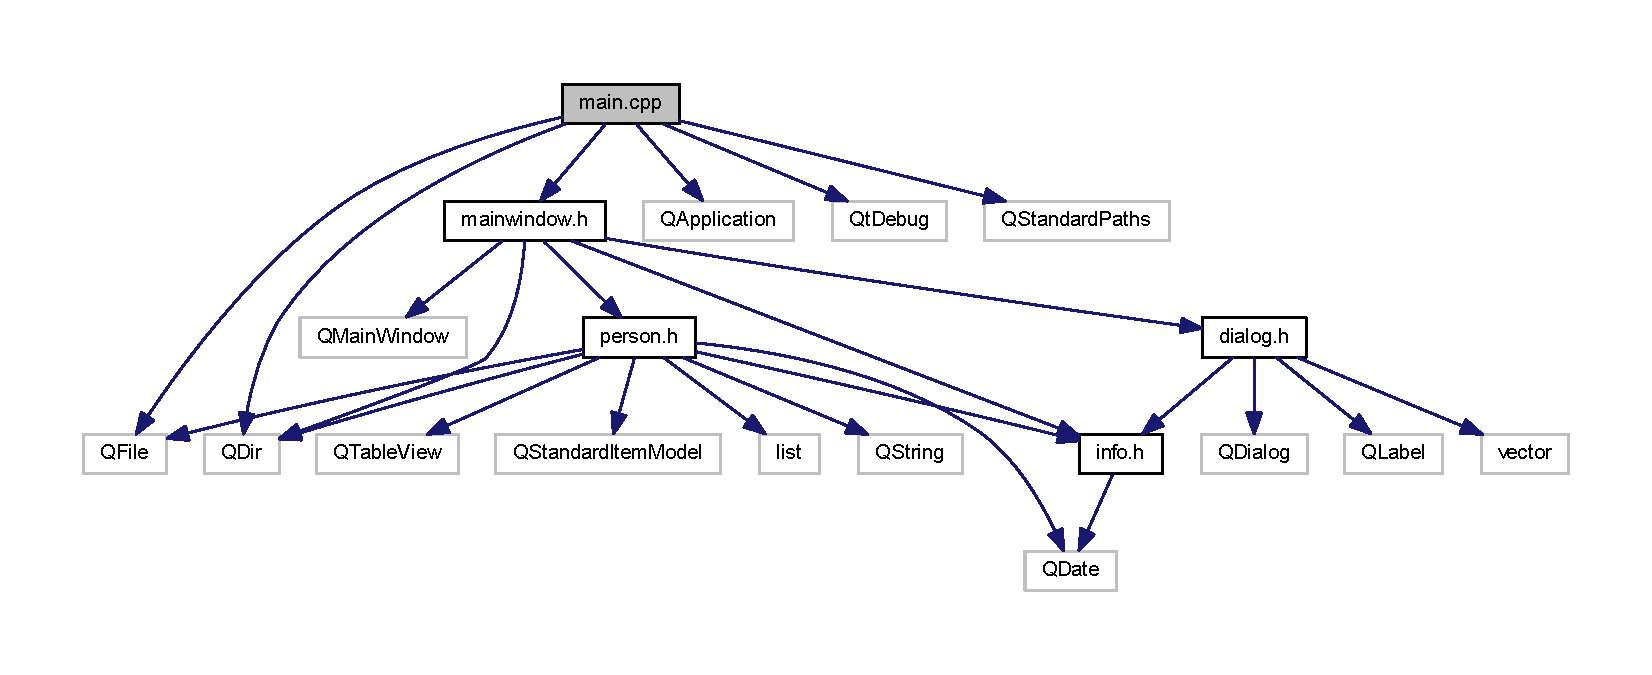
\includegraphics[width=350pt]{main_8cpp__incl}
\end{center}
\end{figure}
\subsection*{Functions}
\begin{DoxyCompactItemize}
\item 
int \hyperlink{main_8cpp_a0ddf1224851353fc92bfbff6f499fa97}{main} (int argc, char $\ast$argv\mbox{[}$\,$\mbox{]})
\end{DoxyCompactItemize}


\subsection{Function Documentation}
\hypertarget{main_8cpp_a0ddf1224851353fc92bfbff6f499fa97}{\index{main.\+cpp@{main.\+cpp}!main@{main}}
\index{main@{main}!main.\+cpp@{main.\+cpp}}
\subsubsection[{main}]{\setlength{\rightskip}{0pt plus 5cm}int main (
\begin{DoxyParamCaption}
\item[{int}]{argc, }
\item[{char $\ast$}]{argv\mbox{[}$\,$\mbox{]}}
\end{DoxyParamCaption}
)}}\label{main_8cpp_a0ddf1224851353fc92bfbff6f499fa97}


Definition at line 8 of file main.\+cpp.


\begin{DoxyCode}
9 \{
10     QApplication a(argc, argv);
11     \hyperlink{class_main_window}{MainWindow} w;
12     
13     QString path(QStandardPaths::writableLocation(QStandardPaths::DataLocation));
14     qDebug() << path;
15     QDir data(path);
16     w.\hyperlink{class_main_window_a44d044deed1ddca8952f59554705e28d}{addPath}(data);
17     \textcolor{keywordflow}{if} (data.exists()) \{
18         qDebug() << \textcolor{stringliteral}{"Trobat"};
19         w.\hyperlink{class_main_window_a6906cd747941813c6da899b18d881473}{loadData}();
20     \}
21     \textcolor{keywordflow}{else} \{
22         qDebug() << \textcolor{stringliteral}{"No s'ha trobat, creant directori"};
23         data.mkpath(path);
24     \}
25     QIcon ico(\textcolor{stringliteral}{"://Images/Hesed.ico"});
26     w.setWindowIcon(ico);
27     w.setWindowTitle(\textcolor{stringliteral}{"Associació Hesed"});
28     w.showMaximized();
29     
30     \textcolor{keywordflow}{return} a.exec();
31 \}
\end{DoxyCode}

\hypertarget{mainwindow_8cpp}{\section{mainwindow.\+cpp File Reference}
\label{mainwindow_8cpp}\index{mainwindow.\+cpp@{mainwindow.\+cpp}}
}
Include dependency graph for mainwindow.\+cpp\+:
\nopagebreak
\begin{figure}[H]
\begin{center}
\leavevmode
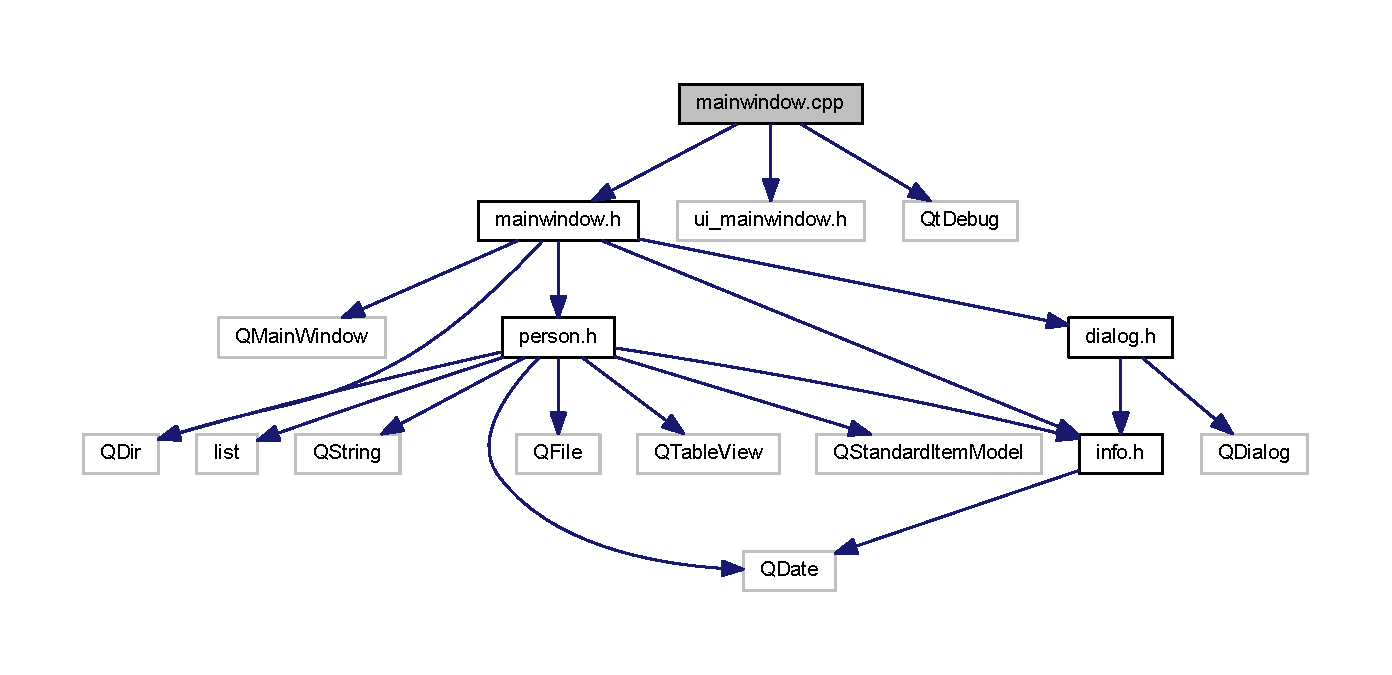
\includegraphics[width=350pt]{mainwindow_8cpp__incl}
\end{center}
\end{figure}

\hypertarget{mainwindow_8h}{\section{mainwindow.\+h File Reference}
\label{mainwindow_8h}\index{mainwindow.\+h@{mainwindow.\+h}}
}
Include dependency graph for mainwindow.\+h\+:\nopagebreak
\begin{figure}[H]
\begin{center}
\leavevmode
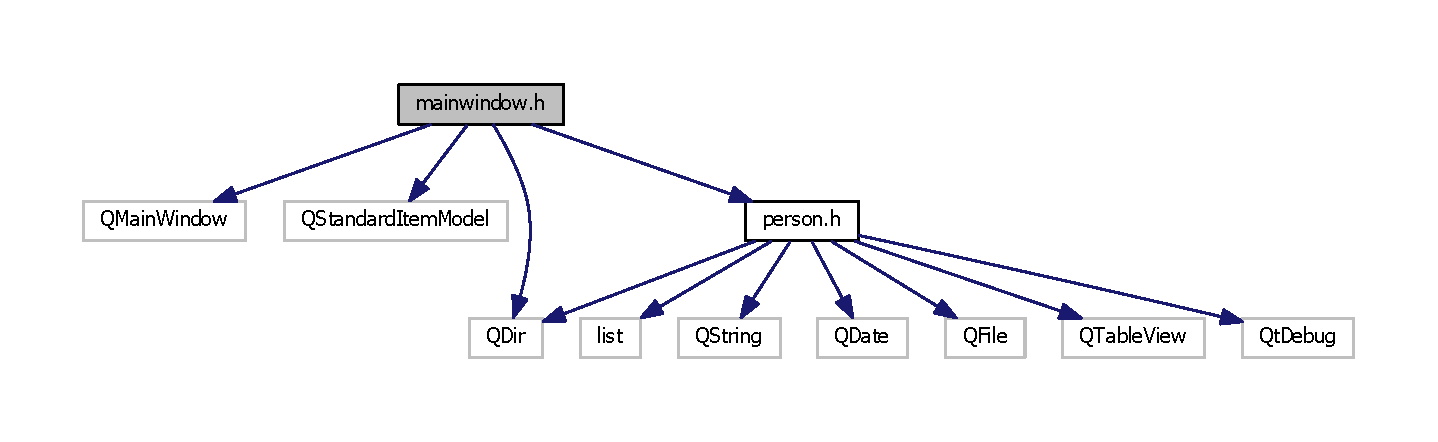
\includegraphics[width=350pt]{mainwindow_8h__incl}
\end{center}
\end{figure}
\subsection*{Classes}
\begin{DoxyCompactItemize}
\item 
class \hyperlink{class_main_window}{Main\+Window}
\begin{DoxyCompactList}\small\item\em Class to show basic information to user. \end{DoxyCompactList}\end{DoxyCompactItemize}
\subsection*{Namespaces}
\begin{DoxyCompactItemize}
\item 
 \hyperlink{namespace_ui}{Ui}
\end{DoxyCompactItemize}

\hypertarget{person_8cpp}{\section{person.\+cpp File Reference}
\label{person_8cpp}\index{person.\+cpp@{person.\+cpp}}
}
Include dependency graph for person.\+cpp\+:
\nopagebreak
\begin{figure}[H]
\begin{center}
\leavevmode
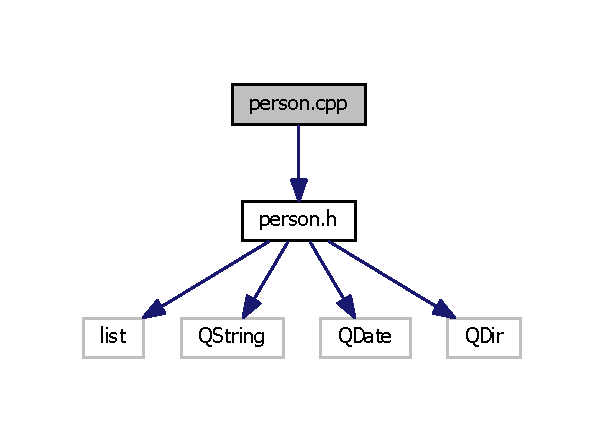
\includegraphics[width=350pt]{person_8cpp__incl}
\end{center}
\end{figure}

\hypertarget{person_8h}{\section{person.\+h File Reference}
\label{person_8h}\index{person.\+h@{person.\+h}}
}
Include dependency graph for person.\+h\+:\nopagebreak
\begin{figure}[H]
\begin{center}
\leavevmode
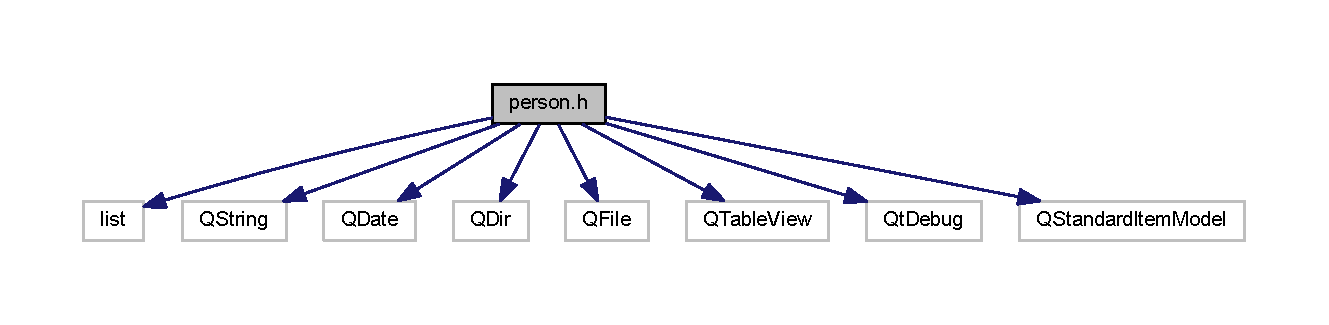
\includegraphics[width=350pt]{person_8h__incl}
\end{center}
\end{figure}
\subsection*{Classes}
\begin{DoxyCompactItemize}
\item 
class \hyperlink{class_person}{Person}
\begin{DoxyCompactList}\small\item\em The \hyperlink{class_person}{Person} Class contains all people basic data. \end{DoxyCompactList}\item 
struct \hyperlink{struct_person_1_1info}{Person\+::info}
\begin{DoxyCompactList}\small\item\em Struct to store basic people information. \end{DoxyCompactList}\item 
struct \hyperlink{struct_person_1_1comp}{Person\+::comp}
\begin{DoxyCompactList}\small\item\em The comp struct is used to sort the info. \end{DoxyCompactList}\end{DoxyCompactItemize}

%--- End generated contents ---

% Index
\newpage
\phantomsection
\addcontentsline{toc}{chapter}{Index}
\printindex

\end{document}
